% Practice Test 11 — Minnesota Edition
% Questions: 30 (19 MC + 11 SA)
% Generated by scripts/generate_practice_tests.py

\begin{practiceQuestion}{1-3-q09}{mc}
\begin{questionText}
Find $k$ from the table.

\begin{center}
\begin{tabular}{|c|c|}
\hline $x$ & $y$ \\ \hline $6$ & $9$ \\ $10$ & $15$ \\ $14$ & $21$ \\ \hline
\end{tabular}
\end{center}
\end{questionText}
\choiceA{$1.5$}
\choiceB{$3$}
\choiceC{$\frac{2}{3}$}
\choiceD{$6$}
\correctAnswer{A}
\explanation{$k = \frac{9}{6} = 1.5$. Check: $\frac{15}{10} = 1.5$ and $\frac{21}{14} = 1.5$.}
\end{practiceQuestion}

\begin{practiceQuestion}{1-5-q11}{mc}
\begin{questionText}
A proportional graph passes through $(5, 12.5)$. What is the equation of this line?
\end{questionText}
\choiceA{$y = 5x$}
\choiceB{$y = 2.5x$}
\choiceC{$y = 12.5x$}
\choiceD{$y = 7.5x$}
\correctAnswer{B}
\explanation{$k = \frac{12.5}{5} = 2.5$, so the equation is $y = 2.5x$.}
\end{practiceQuestion}

\begin{practiceQuestion}{1-6-q13}{mc}
\begin{questionText}
An architect's model uses a scale of $1$ inch $= 3$ feet. If a room in the model is $5.5$ inches long, what is the actual length?
\end{questionText}
\choiceA{$8.5$ feet}
\choiceB{$15$ feet}
\choiceC{$16.5$ feet}
\choiceD{$18$ feet}
\correctAnswer{C}
\explanation{Actual length $= 5.5 \times 3 = 16.5$ feet.}
\end{practiceQuestion}

\begin{practiceQuestion}{2-1-q08}{mc}
\begin{questionText}
$36$ is $45\%$ of what number?
\end{questionText}
\choiceA{$16.2$}
\choiceB{$72$}
\choiceC{$80$}
\choiceD{$90$}
\correctAnswer{C}
\explanation{Divide the part by the percent: $36 \div 0.45 = 80$.}
\end{practiceQuestion}

\begin{practiceQuestion}{2-5-q03}{mc}
\begin{questionText}
A concert ticket costs $\$65$. There is a $15\%$ service fee. What is the total?
\end{questionText}
\choiceA{$\$9.75$}
\choiceB{$\$55.25$}
\choiceC{$\$74.75$}
\choiceD{$\$80.00$}
\correctAnswer{C}
\explanation{$65 \times 1.15 = \$74.75$.}
\end{practiceQuestion}

\begin{practiceQuestion}{2-7-q09}{mc}
\begin{questionText}
If your estimate is exactly correct, what is the percent error?
\end{questionText}
\choiceA{$0\%$}
\choiceB{$1\%$}
\choiceC{$50\%$}
\choiceD{$100\%$}
\correctAnswer{A}
\explanation{If estimated $=$ actual, then $|estimated - actual| = 0$, so percent error $= 0\%$.}
\end{practiceQuestion}

\begin{practiceQuestion}{2-8-q09}{mc}
\begin{questionText}
You buy a $\$120$ jacket. Using a debit card costs $\$120$. Using a credit card at $15\%$ annual interest (paid after $1$ year) costs how much total?
\end{questionText}
\choiceA{$\$120$}
\choiceB{$\$135$}
\choiceC{$\$138$}
\choiceD{$\$150$}
\correctAnswer{C}
\explanation{Interest $= 120 \times 0.15 = \$18$. Total $= 120 + 18 = \$138$.}
\end{practiceQuestion}

\begin{practiceQuestion}{3-1-q08}{mc}
\begin{questionText}
What is the opposite of the opposite of $4$?
\end{questionText}
\choiceA{$-4$}
\choiceB{$0$}
\choiceC{$4$}
\choiceD{$\frac{1}{4}$}
\correctAnswer{C}
\explanation{The opposite of $4$ is $-4$. The opposite of $-4$ is $4$. Taking the opposite twice returns you to the original number.}
\end{practiceQuestion}

\begin{practiceQuestion}{4-1-q27}{gmc}
\begin{questionText}
The diagram below represents an algebraic expression using algebra tiles.

\begin{center}
\begin{tikzpicture}[scale=0.6]
  % x-tiles (rectangles)
  \fill[funBlue!40] (0,0) rectangle (2,1);
  \draw[thick] (0,0) rectangle (2,1);
  \node at (1,0.5) {$x$};
  \fill[funBlue!40] (2.5,0) rectangle (4.5,1);
  \draw[thick] (2.5,0) rectangle (4.5,1);
  \node at (3.5,0.5) {$x$};
  \fill[funBlue!40] (5,0) rectangle (7,1);
  \draw[thick] (5,0) rectangle (7,1);
  \node at (6,0.5) {$x$};
  % unit tiles (squares)
  \fill[funGreen!40] (8,0) rectangle (9,1);
  \draw[thick] (8,0) rectangle (9,1);
  \node at (8.5,0.5) {$1$};
  \fill[funGreen!40] (9.5,0) rectangle (10.5,1);
  \draw[thick] (9.5,0) rectangle (10.5,1);
  \node at (10,0.5) {$1$};
\end{tikzpicture}
\end{center}

Which expression do the tiles represent?
\end{questionText}
\choiceA{$3x + 2$}
\choiceB{$2x + 3$}
\choiceC{$5x$}
\choiceD{$3x \times 2$}
\correctAnswer{A}
\explanation{There are $3$ $x$-tiles and $2$ unit tiles. The expression is $3x + 2$.}
\end{practiceQuestion}

\begin{practiceQuestion}{4-2-q30}{gsa}
\begin{questionText}
The table shows the number of each type of tile in a bag. Write a simplified expression for the total number of tiles.

\begin{center}
\begin{tabular}{|l|c|}
\hline
\textbf{Tile Color} & \textbf{Number of Tiles} \\
\hline
Red & $3n + 4$ \\
\hline
Blue & $2n - 1$ \\
\hline
Green & $n + 5$ \\
\hline
Yellow & $4n - 2$ \\
\hline
\end{tabular}
\end{center}
\end{questionText}
\correctAnswer{$10n + 6$}
\explanation{Add all expressions: $(3n + 4) + (2n - 1) + (n + 5) + (4n - 2)$. Combine variable terms: $3n + 2n + n + 4n = 10n$. Combine constants: $4 - 1 + 5 - 2 = 6$. Total: $10n + 6$.}
\end{practiceQuestion}

\begin{practiceQuestion}{5-2-q22}{sa}
\begin{questionText}
A ride-share app charges $\$2.50$ per mile plus a $\$3.00$ base fee. The total fare was $\$15.50$. How many miles was the ride?
\end{questionText}
\correctAnswer{$5$ miles}
\explanation{$2.50m + 3 = 15.50$. Subtract $3$: $2.50m = 12.50$. Divide by $2.50$: $m = 5$.}
\end{practiceQuestion}

\begin{practiceQuestion}{5-3-q16}{mc}
\begin{questionText}
Solve $8(x + 1) = 48$.
\end{questionText}
\choiceA{$x = 5$}
\choiceB{$x = 6$}
\choiceC{$x = 7$}
\choiceD{$x = \dfrac{47}{8}$}
\correctAnswer{A}
\explanation{Divide by $8$: $x + 1 = 6$. Subtract $1$: $x = 5$. Check: $8(5 + 1) = 8(6) = 48$ \checkmark.}
\end{practiceQuestion}

\begin{practiceQuestion}{5-4-q04}{mc}
\begin{questionText}
Which is the best first step to solve $\dfrac{x}{4} + \dfrac{1}{2} = 3$?
\end{questionText}
\choiceA{Subtract $\frac{1}{2}$ from both sides}
\choiceB{Multiply every term by $4$}
\choiceC{Divide both sides by $4$}
\choiceD{Add $\frac{1}{2}$ to both sides}
\correctAnswer{B}
\explanation{Multiplying every term by $4$ (the LCD) clears the fractions: $x + 2 = 12$.}
\end{practiceQuestion}

\begin{practiceQuestion}{5-5-q14}{mc}
\begin{questionText}
Solve $7 - 2x < 1$.
\end{questionText}
\choiceA{$x < 3$}
\choiceB{$x > 3$}
\choiceC{$x < -3$}
\choiceD{$x > -3$}
\correctAnswer{B}
\explanation{Subtract $7$: $-2x < -6$. Divide by $-2$ and flip: $x > 3$.}
\end{practiceQuestion}

\begin{practiceQuestion}{5-6-q20}{sa}
\begin{questionText}
Solve $-5x + 15 \geq 30$. Describe the graph.
\end{questionText}
\correctAnswer{$x \leq -3$; closed circle at $-3$, shade left}
\explanation{Subtract $15$: $-5x \geq 15$. Divide by $-5$ and flip: $x \leq -3$. Closed circle at $-3$, shade left.}
\end{practiceQuestion}

\begin{practiceQuestion}{6-3-q26}{gmc}
\begin{questionText}
Look at the three segments below. Can they form a triangle?

\begin{center}
\begin{tikzpicture}
  \draw[thick,funBlue] (0,0) -- (2,0);
  \node[below] at (1,0) {$2$ cm};
  \draw[thick,funBlue] (0,-1) -- (3,-1);
  \node[below] at (1.5,-1) {$3$ cm};
  \draw[thick,funBlue] (0,-2) -- (6,-2);
  \node[below] at (3,-2) {$6$ cm};
\end{tikzpicture}
\end{center}
\end{questionText}
\choiceA{Yes, exactly one triangle}
\choiceB{Yes, more than one triangle}
\choiceC{No, because $2 + 3 < 6$}
\choiceD{No, because the sides are all different lengths}
\correctAnswer{C}
\explanation{$2 + 3 = 5 < 6$. The two shorter sides cannot reach across the longest, so no triangle can be formed.}
\end{practiceQuestion}

\begin{practiceQuestion}{6-4-q29}{gsa}
\begin{questionText}
Look at the triangle below. Two sides and the included angle are given. What is the condition type, and is the triangle unique?

\begin{center}
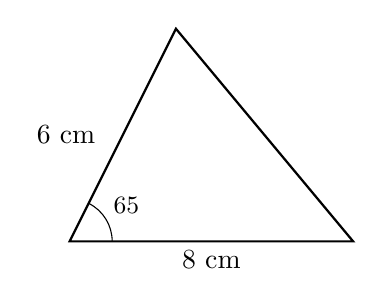
\begin{tikzpicture}[scale=0.9]
  \draw[thick] (0,0) -- (4,0) -- (1.5,3) -- cycle;
  \node[below] at (2,0) {$8$ cm};
  \node[left] at (0.5,1.5) {$6$ cm};
  \draw (0.6,0) arc[start angle=0,end angle=63,radius=0.6];
  \node at (0.8,0.5) {\small $65°$};
\end{tikzpicture}
\end{center}
\end{questionText}
\correctAnswer{SAS; yes, the triangle is unique}
\explanation{Two sides ($8$ cm and $6$ cm) and the included angle ($65°$) give the SAS condition. SAS always produces exactly one unique triangle.}
\end{practiceQuestion}

\begin{practiceQuestion}{6-5-q30}{gsa}
\begin{questionText}
The diagram shows a cube with edge length $6$ cm. A diagonal cut is made from vertex $A$ through the center to the opposite vertex $B$, passing through four faces. What type of shape could this cross-section be?

\begin{center}
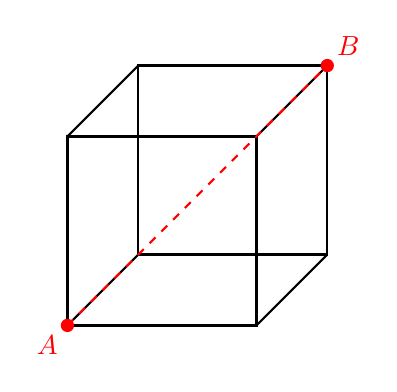
\begin{tikzpicture}[scale=0.6]
  % Front face
  \draw[thick] (0,0) -- (4,0) -- (4,4) -- (0,4) -- cycle;
  % Back face
  \draw[thick] (1.5,1.5) -- (5.5,1.5) -- (5.5,5.5) -- (1.5,5.5) -- cycle;
  % Connecting edges
  \draw[thick] (0,0) -- (1.5,1.5);
  \draw[thick] (4,0) -- (5.5,1.5);
  \draw[thick] (4,4) -- (5.5,5.5);
  \draw[thick] (0,4) -- (1.5,5.5);
  % Diagonal vertices
  \fill[red] (0,0) circle (4pt) node[below left] {$A$};
  \fill[red] (5.5,5.5) circle (4pt) node[above right] {$B$};
  % Diagonal line
  \draw[thick,red,dashed] (0,0) -- (5.5,5.5);
\end{tikzpicture}
\end{center}
\end{questionText}
\correctAnswer{A rectangle}
\explanation{A diagonal cut from one vertex of a cube to the opposite vertex, passing through four faces, creates a rectangular cross-section. The rectangle's dimensions are a face diagonal ($6\sqrt{2}$ cm) by the edge length ($6$ cm).}
\end{practiceQuestion}

\begin{practiceQuestion}{6-6-q07}{mc}
\begin{questionText}
Two vertical angles are $(5x - 20)°$ and $(3x + 10)°$. What is the measure of each angle?
\end{questionText}
\choiceA{$45°$}
\choiceB{$55°$}
\choiceC{$60°$}
\choiceD{$75°$}
\correctAnswer{B}
\explanation{Vertical angles are equal: $5x - 20 = 3x + 10$. Subtract $3x$: $2x - 20 = 10$. Add $20$: $2x = 30$. Divide: $x = 15$. Angle: $5(15) - 20 = 55°$.}
\end{practiceQuestion}

\begin{practiceQuestion}{7-3-q03}{mc}
\begin{questionText}
A circle has a diameter of $12$ inches. What is its area? Use $\pi \approx 3.14$.
\end{questionText}
\choiceA{$37.68$ in$^2$}
\choiceB{$113.04$ in$^2$}
\choiceC{$452.16$ in$^2$}
\choiceD{$144$ in$^2$}
\correctAnswer{B}
\explanation{$r = 12 \div 2 = 6$ in. $A = \pi r^2 = 3.14 \times 36 = 113.04$ in$^2$.}
\end{practiceQuestion}

\begin{practiceQuestion}{7-4-q25}{sa}
\begin{questionText}
A trapezoidal garden has parallel sides of $8$ m and $12$ m, and a height of $5$ m. What is its area?
\end{questionText}
\correctAnswer{$50$ m$^2$}
\explanation{$A = \frac{1}{2}(b_1 + b_2) \times h = \frac{1}{2}(8 + 12) \times 5 = \frac{1}{2} \times 20 \times 5 = 50$ m$^2$.}
\end{practiceQuestion}

\begin{practiceQuestion}{7-5-q10}{mc}
\begin{questionText}
A cube has a surface area of $54$ cm$^2$. What is the area of one face?
\end{questionText}
\choiceA{$6$ cm$^2$}
\choiceB{$9$ cm$^2$}
\choiceC{$18$ cm$^2$}
\choiceD{$27$ cm$^2$}
\correctAnswer{B}
\explanation{A cube has $6$ identical faces. Area of one face $= 54 \div 6 = 9$ cm$^2$.}
\end{practiceQuestion}

\begin{practiceQuestion}{7-6-q25}{sa}
\begin{questionText}
Two rectangular prisms have the same base of $5$ cm by $4$ cm. Prism A is $6$ cm tall and Prism B is $9$ cm tall. What is the difference in their volumes?
\end{questionText}
\correctAnswer{$60$ cm$^3$}
\explanation{$V_A = 5 \times 4 \times 6 = 120$ cm$^3$. $V_B = 5 \times 4 \times 9 = 180$ cm$^3$. Difference: $180 - 120 = 60$ cm$^3$.}
\end{practiceQuestion}

\begin{practiceQuestion}{8-1-q07}{mc}
\begin{questionText}
Which of the following is an example of a biased sample?
\end{questionText}
\choiceA{Randomly selecting $50$ names from a hat containing all student names}
\choiceB{Using a random number generator to pick $30$ employees}
\choiceC{Asking every $10$th person who enters a store}
\choiceD{Surveying only members of the basketball team about school sports}
\correctAnswer{D}
\explanation{Basketball players have strong opinions about sports that may not represent the whole school.}
\end{practiceQuestion}

\begin{practiceQuestion}{8-3-q23}{sa}
\begin{questionText}
What does it mean when two box plots have a large gap between them on a number line?
\end{questionText}
\correctAnswer{The two groups have very different values with little or no overlap}
\explanation{A large gap indicates the groups' data ranges do not overlap much, suggesting a clear difference between the populations.}
\end{practiceQuestion}

\begin{practiceQuestion}{8-4-q19}{sa}
\begin{questionText}
Data: $30, 35, 40, 45, 50$. Find the mean and range.
\end{questionText}
\correctAnswer{Mean $= 40$; Range $= 20$}
\explanation{Mean: $\frac{30+35+40+45+50}{5} = \frac{200}{5} = 40$. Range: $50 - 30 = 20$.}
\end{practiceQuestion}

\begin{practiceQuestion}{8-6-q25}{sa}
\begin{questionText}
A class of $50$ students: $20$ prefer summer, $15$ prefer winter, $10$ prefer fall, $5$ prefer spring. What percent prefer fall?
\end{questionText}
\correctAnswer{$20\%$}
\explanation{$\frac{10}{50} = 0.20 = 20\%$.}
\end{practiceQuestion}

\begin{practiceQuestion}{9-4-q28}{gmc}
\begin{questionText}
Look at the two bags below. Which bag represents a uniform probability model for drawing a marble?

\begin{center}
\begin{tikzpicture}[scale=0.65]
  % Bag 1
  \draw[thick,rounded corners=8pt] (-3,-1.5) rectangle (0,1.5);
  \node[above,font=\bfseries] at (-1.5,1.5) {Bag 1};
  \fill[funRed] (-2.3,0.5) circle (0.3);
  \fill[funRed] (-1.5,0.5) circle (0.3);
  \fill[funBlue] (-0.7,0.5) circle (0.3);
  \fill[funBlue] (-2.3,-0.5) circle (0.3);
  \fill[funGreen] (-1.5,-0.5) circle (0.3);
  \fill[funGreen] (-0.7,-0.5) circle (0.3);
  % Bag 2
  \draw[thick,rounded corners=8pt] (1,-1.5) rectangle (4,1.5);
  \node[above,font=\bfseries] at (2.5,1.5) {Bag 2};
  \fill[funRed] (1.7,0.5) circle (0.3);
  \fill[funRed] (2.5,0.5) circle (0.3);
  \fill[funRed] (3.3,0.5) circle (0.3);
  \fill[funRed] (1.7,-0.5) circle (0.3);
  \fill[funBlue] (2.5,-0.5) circle (0.3);
  \fill[funGreen] (3.3,-0.5) circle (0.3);
\end{tikzpicture}
\end{center}
\end{questionText}
\choiceA{Bag 1 only}
\choiceB{Bag 2 only}
\choiceC{Both bags}
\choiceD{Neither bag}
\correctAnswer{A}
\explanation{Bag 1 has $2$ of each color ($2$ red, $2$ blue, $2$ green), so each color is equally likely — uniform. Bag 2 has $4$ red, $1$ blue, $1$ green — non-uniform.}
\end{practiceQuestion}

\begin{practiceQuestion}{9-6-q17}{mc}
\begin{questionText}
Two spinners are spun. Spinner 1 has sections $\{1, 2, 3\}$ and Spinner 2 has sections $\{A, B\}$. What is the probability of getting $2$ and $A$?
\end{questionText}
\choiceA{$\frac{1}{3}$}
\choiceB{$\frac{1}{5}$}
\choiceC{$\frac{1}{6}$}
\choiceD{$\frac{2}{6}$}
\correctAnswer{C}
\explanation{$P(2) = \frac{1}{3}$, $P(A) = \frac{1}{2}$. $P = \frac{1}{3} \times \frac{1}{2} = \frac{1}{6}$.}
\end{practiceQuestion}

\begin{practiceQuestion}{9-7-q19}{sa}
\begin{questionText}
A simulation uses a coin flip ($50\%$ chance) to model whether it rains on a given day. In $30$ trials, rain occurs $16$ times. What is the experimental probability of rain?
\end{questionText}
\correctAnswer{$\frac{16}{30}$}
\explanation{$P = \frac{16}{30} \approx 0.533$.}
\end{practiceQuestion}
